\documentclass[serif,xcolor=pdftex,dvipsnames,table,hyperref={bookmarks=false,breaklinks}]{beamer}

%%%%%%%%%%%%%%%%
% Change the macros below to configure the title slides
% for your course.
\newcommand{\coursename}{COMPSCI 589}
\newcommand{\instructor}{Benjamin M. Marlin}
\newcommand{\university}{University of Massachusetts Amherst}
\newcommand{\department}{College of Information and Computer Sciences}
%%%%%%%%%%%%%%%%


\newcommand{\settitlecard}[2]{
  \title[\coursename  Lecture #1] 
    {\coursename \\ Lecture #1: #2}
     \author[\instructor]{\instructor}
     \institute[\university]{
     \department\\
     \university
   }
\date{}
}

\newcommand{\maketitlepage}{
  \begin{frame}
  \titlepage
  \center{
    %If you use the slides unmodified, retain the attribution below
    \tiny{Slides by Benjamin M. Marlin (marlin@cs.umass.edu). \\
    \vspace{-1em}Created with support from National Science Foundation Award\# IIS-1350522. 
    %If you modify the slides, please retain the alternate attribution below
    %\tiny{Based on slides by Benjamin M. Marlin (marlin@cs.umass.edu). \\    
    %\vspace{-1em}Created with support from National Science Foundation Award\# IIS-1350522. 
    }                                              
  }  
  \end{frame}
}

\AtBeginSection[]
{
  \begin{frame}<beamer>{Outline}
    \tableofcontents[currentsection,subsectionstyle=hide]
  \end{frame}
}


\newcommand{\cut}[1]{}

\newcommand{\iconbox}[4]{
  \only<#1-#2>{
    \begin{columns}[T]
      \column{0.5in}
           \includegraphics[width=0.5in]{#3}
       \column{3.7in}
            #4
    \end{columns}
    \medskip
    \medskip
    \medskip
  }
}

\mode<presentation>{
  \usepackage{../beamertheme589theme}
  \setbeamercovered{invisible}
}

\mode<handout>{
  \usepackage{../beamertheme589theme}
  \setbeamercovered{transparent}
}


\usepackage[english]{babel}
\usepackage[latin1]{inputenc}
\usepackage{times}
\usepackage[T1]{fontenc}
\usepackage{amsmath}
\usepackage{amssymb}
\usepackage[noend]{algorithmic}
\usepackage{algorithm}
\usepackage{listings}

\renewcommand\mathfamilydefault{\rmdefault}

\newcommand{\setA}{\mathcal{A}}
\newcommand{\setB}{\mathcal{B}}
\newcommand{\setS}{\mathcal{S}}
\newcommand{\setV}{\mathcal{V}}
\DeclareMathOperator*{\union}{\bigcup}
\DeclareMathOperator*{\intersection}{\bigcap}
\DeclareMathOperator*{\Val}{Val}
\newcommand{\mbf}[1]{{\mathbf{#1}}}
\DeclareMathOperator*{\argmax}{arg\,max}
\DeclareMathOperator*{\argmin}{arg\,min}
\DeclareMathOperator*{\sign}{sign}
\newcommand{\deriv}[2]{\frac{\partial{#1}}{\partial{#2}}}


\settitlecard{14}{Data Parallel Programming Abstractions in Spark}

\begin{document}

\maketitlepage

\section{Programming with Spark}
\subsection{Foo}

\begin{frame}[t]{Apache Spark}
\begin{itemize}

\item Apache Spark is a parallel and distributed programming framework that 
adds 
additional parallel abstractions and allows for distributed 
in-memory caching as well as distributed on-disk data access. This makes it 
much faster than MapReduce for ML tasks.

\pause
\center
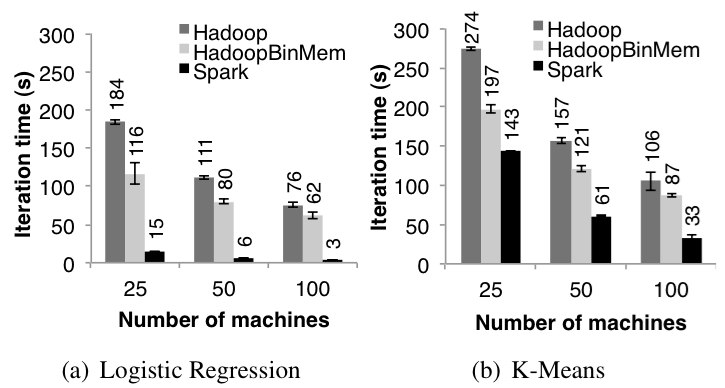
\includegraphics[width=3.4in]{../Figures/spark_vs_hadoop.png}\\
\end{itemize}
\end{frame}

\begin{frame}[t]{Distributed Data Abstraction}
\begin{itemize}

\item Spark's primary abstraction is a data structure called a 
\textit{resilient distributed data set} or RDD.

\pause\item An RDD is a read-only partitioned collection of objects that is 
stored across one or more nodes in a Spark cluster.

\pause\item RDDs are created by applying a sequence of \textit{transformations} 
to data. Results are obtained by applying \textit{actions} to RDDs.

\pause\item The Spark system keeps track of the transformations used to create 
each partition of an RDD and can dynamically re-generate lost partitions on 
other cluster nodes. This makes it very fault-tolerant. 

\end{itemize}
\end{frame}

\begin{frame}[t]{Creating RDDs from Data}

\begin{itemize}

\pause\item An RDD is initially created from a root Spark context object. 

\pause \item Supported methods include $textFile(path)$ to create an RDD from a 
text file (or a directory of files), and $parallelize(data)$ to partition an 
existing collection.

\pause \item Spark can run over a regular file system or the Hadoop file system
(HDFS), which provides on-disk distributed storage.


\end{itemize}
\end{frame}

\begin{frame}[t]{Parallel Programming Abstractions: Transformations}

For the reasons covered last class, transformations on RDDs are 
specified through parallel programming abstractions with functional semantics:

\begin{itemize}
\item $map(f)$:  Return a new distributed dataset formed by passing each 
element of the source through a function $f$.

\pause\item $flatMap(f)$:   Similar to map, but each input item can be 
mapped to 0 or more output items (so $f$ should return a list rather than a 
single item). 

\pause\item $filter(f)$:  Return a new dataset formed by selecting those 
elements of the source on which $f$ returns true.

\pause\item $reduceByKey(func, [numTasks])$:   When called on a dataset of $(K, 
V)$ pairs, returns a dataset of $(K, V)$ pairs where the values for each key 
are aggregated using the given reduce function $f$, which must be of type 
$(V,V) => V$. 
\end{itemize}

\end{frame}

\begin{frame}[t]{Parallel Programming Abstractions: Transformations}


\begin{itemize}
\item Transformation use lazy evaluation.

\pause\item No transformations are applied until you call an action on an RDD.

\pause\item Why is Spark implemented in this way?

\end{itemize}

\end{frame}


\begin{frame}[t]{Parallel Programming Abstractions: Actions}

Actions on RDDs return actual values to the Spark master process:

\begin{itemize}

\item $collect()$:    Return all the elements of the dataset as an array to 
the driver program. This is usually useful after a filter or other operation 
that returns a sufficiently small subset of the data. 

\pause\item $reduce(f)$:    Aggregate the elements of the dataset using a 
function $f$ (which takes two arguments and returns one). The function 
should be commutative and associative so that it can be computed correctly in 
parallel. 

\pause\item$first()$:         Return the first element of the dataset.

\pause\item$take(n)$:        Return an array with the first $n$ elements of the 
dataset. 

\pause\item$saveAsTextFile(path)$:    Write the elements of the dataset as a 
text file (or set of text files) in a given directory in the filesystem.

\end{itemize}

\end{frame}

\begin{frame}[t]{Spark API}

The Python Spark RDD API is fully documented here:

\center
\url{http://spark.apache.org/docs/latest/api/python/pyspark.html\#pyspark.RDD}

\end{frame}

\begin{frame}[t]{Mixing Imperative and Functional Programming}

\begin{itemize}

\item Importantly, programs written using Spark can mix regular imperative
programming with the functional parallel programming abstractions that Spark 
provides.

\pause\item All code in the Spark master process and in individual functions $f$
passed to Spark can be regular single-threaded imperative code.

\end{itemize}

\pause
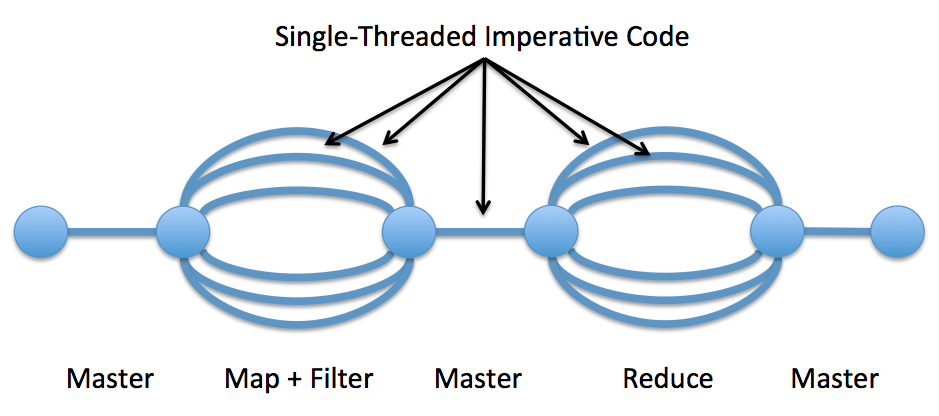
\includegraphics[width=4in]{../Figures/spark_flow.png}

\end{frame}

\begin{frame}[t]{Spark and Numpy}

\begin{itemize}

\item We can use any Python data types in RDDs and any Python 
library functions inside the functions we pass to Spark transformations and 
actions. In particular, we can use Numpy functions.

\pause\item A common operation is to map the rows of an RDD to Numpy arrays
so that we can apply Numpy operations to them within Spark map and reduce operations.

\end{itemize}

\end{frame}


\begin{frame}[t]{In Memory Caching of RDDs}

\begin{itemize}

\item The main advantage of Spark over MapReduce/Hadoop is that
it has the ability to cache RDDs in memory on remote cluster nodes.

\pause\item In the absence of caching, an RDD is recomputed from the
base data from scratch including all transformations each time an action
is called on it.

\pause\item Caching makes Spark much faster than Hadoop for iterative algorithms
or repeated queries since the data doesn't need to be read of disk for each
iteration or query.

\pause\item An RDD can be marked for caching by calling $cache()$ on it. 


\end{itemize}

\end{frame}


\begin{frame}[t]{Spark and Machine Learning}

\begin{itemize}

\item Since the computationally intensive part of most machine learning
computations on big data involves computations that are embarrassingly parallel
with respect to the data, Spark can be a great fit.

\pause \item To re-write a Python implementation of a  method like 
logistic regression learning or prediction, we need to replace the loops 
over the data with map and reduce steps.

\pause \item Let's look at the fundamental operation of classifying data cases
contained in the rows of an RDD using a linear classifier implemented with Spark:

$$w^Tx + b = \sum_{i=1}^D w_ix_i +b >0$$

\end{itemize}

\end{frame}


\end{document}
